% !TEX root = ../main.tex
%
\chapter{System Design and Implementation}
\label{sec:system}

A very important part of this thesis is the Synthetic Discussion Framework (SDF), a lightweight, specialized python library which supports the automatic creation of dialogues through LLMs. In this section we explain in detail the initial requirements for this framework, why commercially-available alternatives do not fit these requirements (Section \ref{sec:system:requirements}), the general design and concept (Section \ref{sec:system:design}), and finally the actual implementation (Section \ref{sec:system:implementation}) of the new framework.

\section{Requirements}
\label{sec:system:requirements}

%TODO: add LLM annotators

The requirements for the SDF were not obtained by standard Requirement Solicitation procedures. Instead, they were iteratively solicited during weekly meetings. Thus, no formal document detailing them exists. 

However, the interested stakeholders in the context of the wider research effort, ultimately decided on a combination of the below requirements. We denote the SDF as "the system" for this section.

Functional requirements:
\begin{enumerate}
	\item The system must support multiple LLM types, with potentially different libraries handling them.
	\item The system must support a conversation with at least two LLM users.
	\item The system must support socio-demographic backgrounds (SDBs) to be given to LLM users.
	\item The system must support the existence and absence of a third LLM user, posing as a moderator.
	\item The moderator must be able to intervene at any point in the conversation.
	\item The moderator must be able to "ban" users, preventing them from further commenting.
	\item The output of the system must be serializable and easily parsable.
	\item The system must support automated annotation.
\end{enumerate}

Non functional requirements:
\begin{enumerate}
	\item The system must be able to be ran locally, with scarce computational resources.
	\item The system must be accessed through a simple and flexible API.
	\item The system must be able to automatically produce a large amount of synthetic discussions in a timeframe of hours.
	\item The system must support large-scale data annotation.
	\item The system must support a diverse and flexible array of annotation criteria.
\end{enumerate}

Current LLM discussion frameworks such as Concordia \cite{Vezhnevets2023GenerativeAM} and LangChain \cite{langchain} fit, or can be made to fit, all functional requirements listed above. They however fail at all three non-functional requirements, as they are industrial-grade frameworks, meant for a diverse set of business use-cases making, their API convoluted. Of course, this could be circumvented by employing the Adapter pattern \cite{gamma1995design}. The problem then would be that their internal components frequently necessitate computer resources (dedicated RAM, GPU VRAM e.t.c.) which, for a smaller application such as ours, will most likely not be used to their fullest.

Thus the solution of building our own framework is the only practical way of satisfying all the requirements above.



\section{System Design}
\label{sec:system:design-system}

The SDF is comprised of two main functions; Synthetic Dialogue Creation and Automatic Dialogue Annotation. In this section, we will explain how these two functions work conceptually and what their goals are.


\subsection{Synthetic Dialogue Creation}
\label{ssec:system:creation}

The simplest form of conversation is one between two actors. While the SDF is capable at holding conversations over an arbitrary number of users, for the purposes of this example we will assume only two users are present, as was the case in our experiments. We also add a third actor, the Moderator, who oversees the conversation. An overview of the conversation loop can be found in Figure \ref{fig::conversation}.

\begin{figure}
	\centering
	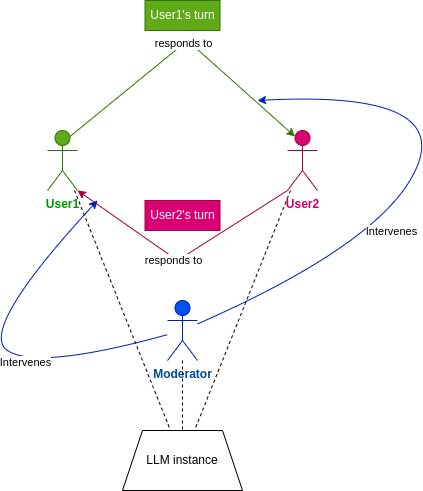
\includegraphics[width=8cm]{conversation_graph_light.png}
	\caption{The conversation loop on which the SDF operates. Can be generalized for N users and 0 or 1 moderators.}
	\label{fig::conversation}
\end{figure}

The two Users and the Moderator are all controlled by the same LLM instance; we only change the system prompt when each takes its turn to speak. The prompts are comprised of five parts:

\begin{itemize}
	\item \textbf{Name}, the name of the actor, used for other actors to refer ro him in-conversation.
	\item \textbf{Role}, the role of the actor within the conversation (user, moderator).
	\item \textbf{Attributes}, a list of actor attributes, primarily used for giving the actor an SDB.
	\item \textbf{Context}, information known to all users.
	\item \textbf{Instructions}, potentially unique to each actor. 
\end{itemize}


\subsection{Automated Dialogue Annotation}
\label{ssec:system:annotation}

As per the non-functional requirements of Section \ref{sec:system:requirements}, we need a mechanism which can automatically annotate already-executed conversations. This could be achieved by using specialized classification models such as a model for toxicity classification, another for argument quality, and so on. However, these usually differ not only on their exact architecture, but also on their fundamental type; for instance, in toxicity classification, competitive models can be ML-based instead of DL-based \cite{anjum2024hate}. Using a diverse set of specialized models, with their own libraries, preprocessing requirements and effectiveness would severely restrict our ability to rapidly change annotation criteria at-scale. To bypass this restriction, we can use LLMs to also handle the annotation step. LLM inference is practically constant-time with a fixed input length, since adding a new annotation metric would only impose a computational penalty equal to the output's increased number of tokens - which is negligible. 

Using LLMs as annotators imposes both a challenge and an opportunity, since annotations are no longer objective (unlike traditional ML and even DL models, we can't explain a LLM's decision). Thus, we are faced with two different approaches:

\begin{itemize}
	\item Attempt to find a prompt which produces results closer to what would be expected of a human annotator.
	\item Lean into the subjectiveness of LLM decision-making and use many LLM annotators, each with a different SDB, then use inter-annotator analysis techniques.
\end{itemize}

In this thesis, we use the second option.

We re-use the conversation paradigm of Section \ref{ssec:system:creation} to facilitate annotation. One pseudo-actor is the system, which outputs comments made in a conversation one-by-one. The other is a LLM actor which responds with the classification rating for each comment (toxicity in these experiments).  We use a context window of 4 for the annotator, that is for each comment the annotator can see the 4 preceding comments of the conversation. The annotation loop is succinctly demonstrated in Figure \ref{fig::annotation}.

\begin{figure}
	\centering
	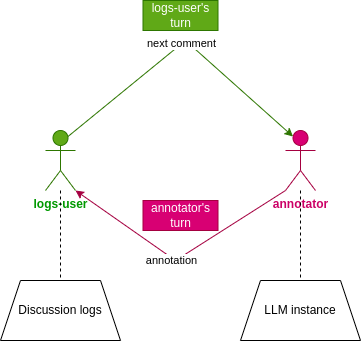
\includegraphics[width=8cm]{annotation_graph_light.png}
	\caption{The annotation loop on which the SDF operates. Note the purposeful similarity of the function to Figure \ref{fig::conversation}.}
	\label{fig::annotation}
\end{figure}


\section{Prompt Design}
\label{sec:system:design-prompt}

Our user instruction prompts in general were designed with the following criteria in mind:

\begin{itemize}
	\item Many people are unwilling to change opinions during online discussions.
	
	\item Personal attacks are common \cite{dekock2022disagree}.
	
	\item Anonymity makes people more likely assume other participants are not arguing in good faith, especially in toxic environments \cite{Avalle2024PersistentIP}.
	
	\item People are not told what to believe when entering a discussion, but form opinions based on (besides many other factors) their SDB.  %TODO citation needed?
	
\end{itemize}

Thus, user prompts are designed to promote toxicity, controversy and confrontation.

On the other hand, our moderator prompts were largely based on the eCornell moderator manual \cite{Cornell_eRulemaking2017} which, among others, emphasizes the following guidelines:

\begin{itemize}
	\item The moderator must remain neutral and impartial. 
	
	\item Responses should be briefly reflected upon before being posted.
	
	\item Questions posed by the moderator must be purposeful, as if they have one chance to interact with the user. They can rephrase a user's point if they do not understand it.
	
	\item Language should be short and simple.
\end{itemize}

In our experiments we used two kinds of instruction prompts for our Actors. One is a "standard" prompt summarizing the guidelines above (Section \ref{ssec:system:vanilla-prompt}). The other formulates the discussion as a scorable, non-zero sum game where the users and the moderator attempt to accomplish conflicting goals (Section \ref{ssec:system:game-prompt}.

\subsection{Vanilla prompts}
\label{ssec:system:vanilla-prompt}

\subsection{"Moderation Game" prompts}
\label{ssec:system:game-prompt}



\section{Implementation}
\label{sec:system:implementation}

\subsection{Synthetic Discussion Library}
\label{ssec:system:library}

The SDF is at its core based on the Synthetic Discussion Library (SDL) around which the rest of the framework operates. The library is written in Python, contains 4 distinct modules, and is based on Object Oriented Programming (OOP) principles.

Each of these modules contains classes and supporting code for a specific function. In brief:

\begin{itemize}
	\item \textbf{models.py} holds Adapter classes \cite{gamma1995design} which enable the framework to uniformly access almost any LLM instance regardless of type (as long as a suitable subclass is created).
	
	\item \textbf{actors.py} which holds Wrapper classes \cite{gamma1995design}, containing Model Adapter classes from \textbf{models.py} and provide them with prompt templates.
	
	\item \textbf{conversation.py} uses Actor classes in order to execute and serialize the conversation.
\end{itemize}

The library additionally provides the \textbf{annotator.py} and \textbf{util.py} modules which are self explanatory.


\subsection{Framework entry-points}
\label{ssec:system:entrypoints}

The framework provides a variety of APIs to access the SDL from the more standardized (which necessitate no programming) to the more flexible (direct access to the library's public API). These are:

\begin{itemize}
	\item Automated python scripts which, when given a JSON configuration file, begin a batch production of automated discussions.
	
	\item Jupyter notebooks with explanatory high-level documentation, which are used for on-boarding users to the framework and quick experimentation.
	
	\item The exported SDL itself.
\end{itemize}


\subsection{High-level view of the system}
\label{ssec:system:overview}

A high-level overview of the system can be found in Figure \ref{fig::system}. The configurations (\textcolor{green}{green shapes}) can be provided by either JSON files or programmatically, depending on the entry-point (\textcolor{blue}{blue shapes}) used. 

The procedure described in the figure, enables us to produce a large amount of data, annotate them, analyze them, and produce concrete results (graphs, statistical tests e.t.c.) with little-to-no manual intervention. Subsequently, these results enable us to change the prompts used by the Actors to refine results or test new hypotheses.

Each processing step (\textcolor{violet}{pink shapes}) additionally creates entries on our generated dataset, be it the conversation logs with rich meta-data (\textcolor{violet}{"Generate Conversation"}), multi-annotator, multi-dimensional annotations (\textcolor{violet}{"Generate Annotation"}) or controversial comments (\textcolor{violet}{"Data Analysis"}).

\begin{figure}
	\centering
	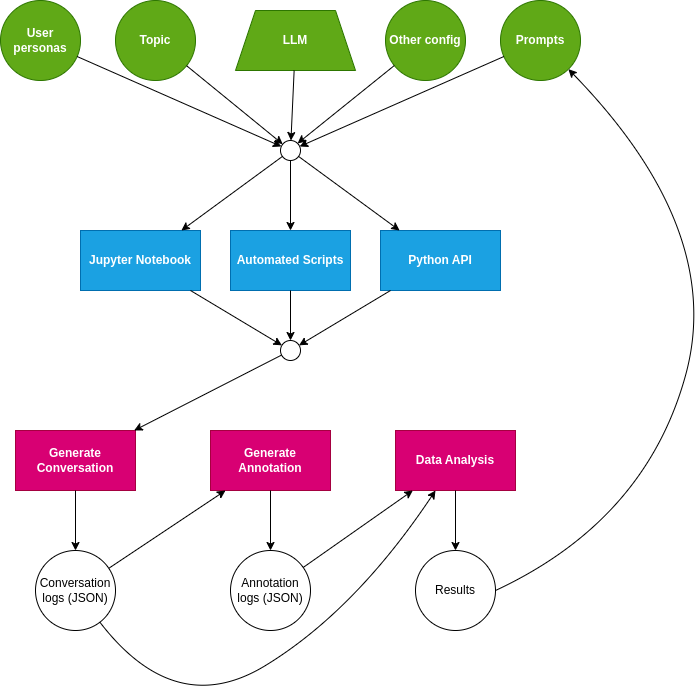
\includegraphics[width=12cm]{system_light.png}
	\caption{An abstract view of the SDF. \textcolor{green}{Green shapes} represent various configurations, \textcolor{blue}{blue shapes} entry points (see Section \ref{ssec:system:entrypoints}), \textcolor{violet}{pink ones} processes delegated to the SDL, and \textbf{white} ones exported data.}
	\label{fig::system}
\end{figure}



\subsection{Technical Details}
\label{ssec:system:details}

The LLM used is the LLaMa2-13B GGUF quantized version. We use the llama\_cpp python library to load and interact with the model. Details on the environment, software and OS compatibility, as well as low-level decisions and optimizations, we recommend checking the project's GitHub repository \footnote{\url{https://github.com/dimits-ts/llm_moderation_research}}.

